\section{Language Semantics for Evaluation} \label{sec:language-semenatics} \btc{Hvad vil I bruge dette afsnit til ?}
The behaviour of programming languages can be difficult to validate. To remedy this, formal semantics can be employed to specify and verify program behaviour. In the field of programming-language technologies, several different notations for such semantics have emerged. The goal of semantics is to provide a specification that a programming language\footnote{These semantics can also be used to specify programs, but are most often used to verify languages.} can be verified. 

\quoteWithCite{Programming language semantics is the study of mathematical models of and methods for describing and reasoning about the behaviour of programs.}{Hans Hüttel}{huttel2010transitions}

Formal methods are used to test the language before and during language implementation \cite{hierons2009using}.  Thus verified code should be more likely to run correctly, furthermore specification and verification may also expose errors in the programmers understanding of the code. This is the property that drives demand for formal specification of programming languages. 

\begin{figure}[H]
    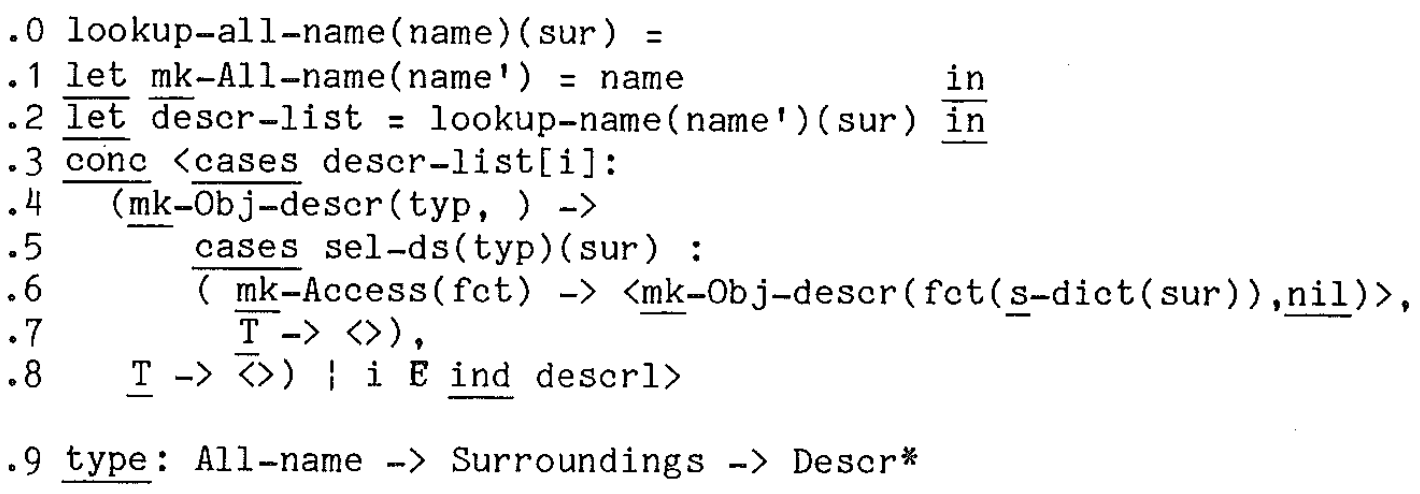
\includegraphics[width=.95\textwidth]{images/vdm-lookup-all-name.png}
    \caption{Ada Static Semantics Fragment \cite{sestoft:isola}}
    \label{fig:ada-semantic}
\end{figure}

However, some formal-specification notations are very similar to functional programming languages, this can be seen in \figureref{ada-semantic}. Therefore Peter Sestoft has explored the idea of using a functional language as specification and implementation \cite{sestoft:isola}. The general idea is that the specification and implementation can, in some cases, be the one and the same. However Sestoft also highlights some cases where specification and implementation cannot be united as of yet.

These findings mean that functional programming can also be used to automate part of the verification process. Sestoft found errors in the Ada partial specification when he implemented the specification in F\#, this can be seen in \lstref{ada-fsh-impl}. These errors include spelling mistakes and incorrect argument order among other things.

\begin{lstlisting}[language=fsharp, caption={Sestoft's F\# Implementation of Ada \cite{sestoft:isola}},label={lst:ada-fsh-impl}]
let lookup_all_name (All_name(name') : All_name) (sur : Surroundings)
                    : seq<Descr> =
    seq { for di in lookup_name(name')(sur) do
            match di with
            | Obj_descr { s_tp = { s_ds = Some (Access {s_map = fct }) } }
                -> yield Obj_descr { s_tp = fct(sur.s_dict); s_con = None }
            | _ -> ()
        }
\end{lstlisting}

This can be employed in game development to rapidly and correctly implement small \acp{DSL}. Such \acp{DSL} allow non-programmer domain experts to produce code \cite{beyak2011saga}. The production of such \acp{DSL} can be costly and may require even more resources to maintain and adapt to other games. However, if a game engine supports function programming this can be utilised to develop the \acp{DSL}.
